\documentclass[aspectratio=169]{beamer}
\usetheme{default}
\usefonttheme{professionalfonts}
\usepackage[T1]{fontenc}
\usepackage{lmodern}
\usepackage{amsmath,amssymb,mathtools}
\usepackage{array,booktabs,graphicx,microtype}
\usepackage{hyperref}
\usepackage{tikz}
\setbeamertemplate{navigation symbols}{}
\setbeamertemplate{headline}{%
  \leavevmode%
  \hbox{%
    \begin{beamercolorbox}[wd=.78\paperwidth,ht=2.6ex,dp=1.1ex,leftskip=1.6em]{frametitle}%
      \usebeamerfont{headline}\insertshorttitle%
    \end{beamercolorbox}%
    \begin{beamercolorbox}[wd=.22\paperwidth,ht=2.6ex,dp=1.1ex,rightskip=1.6em]{frametitle}%
      \hfill\raisebox{-.55ex}{\includegraphics[height=2.4ex]{units.jpg}}%
    \end{beamercolorbox}%
  }%
  \vskip.2ex\hrule height .3pt%
}
\setbeamertemplate{footline}{%
  \leavevmode%
  \hbox{%
    \begin{beamercolorbox}[wd=.82\paperwidth,ht=2.2ex,dp=.8ex,leftskip=1.6em]{frametitle}%
      \usebeamerfont{headline}\href{mailto:sylvio.barbonjunior@units.it}{sylvio.barbonjunior@units.it}%
    \end{beamercolorbox}%
    \begin{beamercolorbox}[wd=.18\paperwidth,ht=2.2ex,dp=.8ex,rightskip=1.6em]{frametitle}%
      \hfill\insertframenumber/\inserttotalframenumber%
    \end{beamercolorbox}%
  }%
}
\setbeamercolor{normal text}{fg=black,bg=white}
\setbeamercolor{frametitle}{fg=black,bg=white}
\setbeamercolor{title}{fg=black}
\setbeamercolor{structure}{fg=black}
\setbeamerfont{headline}{size=\scriptsize}
\setbeamertemplate{itemize item}{--}
\setbeamertemplate{itemize subitem}{\textbullet}
\graphicspath{{figures/}}
\definecolor{contentblue}{RGB}{50,83,116}
\definecolor{presentationteal}{RGB}{38,125,117}
\definecolor{usergold}{RGB}{178,119,28}

\newcommand{\ContentIcon}{%
\tikz[baseline=-.55ex,x=1ex,y=1ex,line width=.12ex]{%
  \draw[contentblue,rounded corners=.15ex] (0,0) rectangle (1.55,1.9);
  \draw[contentblue] (.48,1.72) rectangle (1.08,1.98);
  \foreach \y in {.45,.95,1.45}{%
    \draw[contentblue] (.25,\y) -- (.42,\y-.17) -- (.72,\y+.18);
    \draw[contentblue] (.88,\y) -- (1.32,\y);
  }%
}}
\newcommand{\PresentationIcon}{%
\tikz[baseline=-.55ex,x=1ex,y=1ex,line width=.12ex]{%
  \draw[presentationteal,rounded corners=.12ex] (0,0) rectangle (1.75,1.9);
  \draw[presentationteal] (.22,1.18) rectangle (.72,1.58);
  \draw[presentationteal] (.9,1.45) -- (1.48,1.45);
  \draw[presentationteal] (.9,1.18) -- (1.48,1.18);
  \draw[presentationteal] (.25,.28) -- (.25,.82);
  \draw[presentationteal] (.55,.28) -- (.55,.6);
  \draw[presentationteal] (.85,.28) -- (.85,.98);
  \draw[presentationteal] (1.15,.28) -- (1.15,.72);
}}
\newcommand{\UserIcon}{%
\tikz[baseline=-.55ex,x=1ex,y=1ex,line width=.12ex]{%
  \draw[usergold] (.75,1.35) circle (.32);
  \draw[usergold,rounded corners=.35ex] (.15,.05) rectangle (1.35,.92);
  \draw[usergold] (1.55,1.42) -- (2.05,1.42);
  \draw[usergold] (1.65,1.16) -- (2.15,1.16);
}}
\newcommand{\PerspectiveTag}[2]{\raisebox{-.2ex}{#1}\,\textbf{#2}}
\newcommand{\xdel}[1]{x^{\mathrm{del}(#1)}}
\newcommand{\xkeep}[1]{x^{\mathrm{keep}(#1)}}
\newcommand{\PerspectiveLegend}{%
  \PerspectiveTag{\ContentIcon}{Content}\hspace{1.4em}%
  \PerspectiveTag{\PresentationIcon}{Presentation}\hspace{1.4em}%
  \PerspectiveTag{\UserIcon}{User}%
}
\newcommand{\HierarchyHeader}[4]{%
  {\scriptsize
  \begin{tabular}{@{}>{\raggedright\arraybackslash}p{.22\linewidth}>{\raggedright\arraybackslash}p{.29\linewidth}>{\raggedright\arraybackslash}p{.39\linewidth}@{}}
  \textbf{Perspective:} \PerspectiveTag{#1}{#2} &
  \textbf{Property:} #3 &
  \textbf{Question:} #4
  \end{tabular}}%
  \vspace{.2em}\hrule\vspace{.4em}%
}
\newcommand{\TradeoffHeader}[7]{%
  {\scriptsize
  \begin{tabular}{@{}>{\raggedright\arraybackslash}p{.28\linewidth}>{\raggedright\arraybackslash}p{.28\linewidth}>{\raggedright\arraybackslash}p{.34\linewidth}@{}}
  \textbf{A:} \PerspectiveTag{#1}{#2}: #3 &
  \textbf{B:} \PerspectiveTag{#4}{#5}: #6 &
  \textbf{Relation:} #7
  \end{tabular}}%
  \vspace{.2em}\hrule\vspace{.4em}%
}

\title[Evaluating Explainable AI: From Quality Properties to Metrics]{Evaluating Explainable AI}
\subtitle{From Quality Properties to Metrics}
\author[Sylvio Barbon Junior]{\texorpdfstring{Sylvio Barbon Junior\\\href{mailto:sylvio.barbonjunior@units.it}{sylvio.barbonjunior@units.it}}{Sylvio Barbon Junior, sylvio.barbonjunior@units.it}}
\institute{Research seminar}
\date{2026}
\titlegraphic{
\includegraphics[height=1.15cm]{units.jpg}}

\begin{document}
\frame{\titlepage}
\begin{frame}{A provocation}
\centering
\Large ``SHAP is better than LIME.''\\[1em]
\normalsize Better according to what?\\[0.5em]
Faithfulness? Stability? Compactness? Human usefulness?
\end{frame}

\begin{frame}{Different explainers, different explanation objects}
\small
\centering
Iris instance, predicted class: \textit{virginica}. Simulated local scores.

\vspace{.8em}
\begin{columns}[T,onlytextwidth]
\column{.31\textwidth}
\centering
\textbf{SHAP feature rank}
\vspace{.25em}

\resizebox{\linewidth}{!}{%
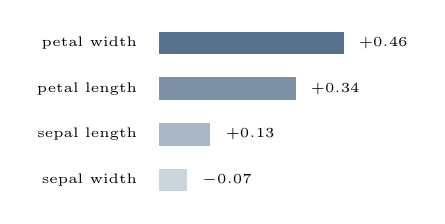
\begin{tikzpicture}[x=1cm,y=.58cm]
  \node[font=\tiny,anchor=east,align=right] at (1.55,3.5) {petal width};
  \fill[contentblue!82] (1.7,3.25) rectangle (4.05,3.75);
  \node[font=\tiny,anchor=west] at (4.12,3.5) {$+0.46$};
  \node[font=\tiny,anchor=east,align=right] at (1.55,2.5) {petal length};
  \fill[contentblue!64] (1.7,2.25) rectangle (3.44,2.75);
  \node[font=\tiny,anchor=west] at (3.51,2.5) {$+0.34$};
  \node[font=\tiny,anchor=east,align=right] at (1.55,1.5) {sepal length};
  \fill[contentblue!42] (1.7,1.25) rectangle (2.36,1.75);
  \node[font=\tiny,anchor=west] at (2.43,1.5) {$+0.13$};
  \node[font=\tiny,anchor=east,align=right] at (1.55,.5) {sepal width};
  \fill[contentblue!25] (1.7,.25) rectangle (2.06,.75);
  \node[font=\tiny,anchor=west] at (2.13,.5) {$-0.07$};
\end{tikzpicture}
}

\column{.32\textwidth}
\centering
\textbf{LIME local rule rank}
\vspace{.25em}

\resizebox{\linewidth}{!}{%
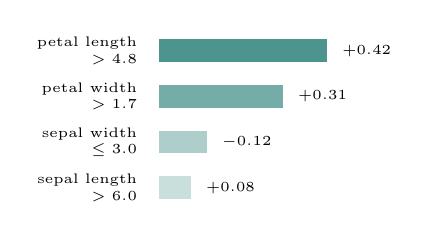
\begin{tikzpicture}[x=1cm,y=.58cm]
  \node[font=\tiny,anchor=east,align=right] at (1.85,3.5) {petal length\\$>4.8$};
  \fill[presentationteal!82] (2.0,3.25) rectangle (4.14,3.75);
  \node[font=\tiny,anchor=west] at (4.21,3.5) {$+0.42$};
  \node[font=\tiny,anchor=east,align=right] at (1.85,2.5) {petal width\\$>1.7$};
  \fill[presentationteal!64] (2.0,2.25) rectangle (3.58,2.75);
  \node[font=\tiny,anchor=west] at (3.65,2.5) {$+0.31$};
  \node[font=\tiny,anchor=east,align=right] at (1.85,1.5) {sepal width\\$\leq3.0$};
  \fill[presentationteal!38] (2.0,1.25) rectangle (2.61,1.75);
  \node[font=\tiny,anchor=west] at (2.68,1.5) {$-0.12$};
  \node[font=\tiny,anchor=east,align=right] at (1.85,.5) {sepal length\\$>6.0$};
  \fill[presentationteal!25] (2.0,.25) rectangle (2.41,.75);
  \node[font=\tiny,anchor=west] at (2.48,.5) {$+0.08$};
\end{tikzpicture}
}

\column{.35\textwidth}
\centering
\textbf{DPG LRC predicate rank}
\vspace{.25em}

\resizebox{\linewidth}{!}{%
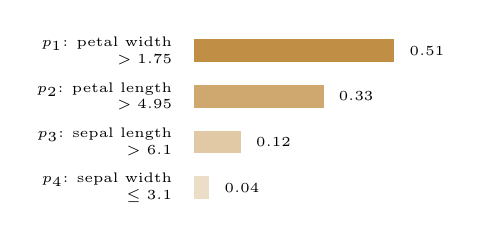
\begin{tikzpicture}[x=1cm,y=.58cm]
  \node[font=\tiny,anchor=east,align=right] at (2.18,3.5) {$p_1$: petal width\\$>1.75$};
  \fill[usergold!82] (2.33,3.25) rectangle (4.88,3.75);
  \node[font=\tiny,anchor=west] at (4.95,3.5) {$0.51$};
  \node[font=\tiny,anchor=east,align=right] at (2.18,2.5) {$p_2$: petal length\\$>4.95$};
  \fill[usergold!64] (2.33,2.25) rectangle (3.98,2.75);
  \node[font=\tiny,anchor=west] at (4.05,2.5) {$0.33$};
  \node[font=\tiny,anchor=east,align=right] at (2.18,1.5) {$p_3$: sepal length\\$>6.1$};
  \fill[usergold!40] (2.33,1.25) rectangle (2.93,1.75);
  \node[font=\tiny,anchor=west] at (3.00,1.5) {$0.12$};
  \node[font=\tiny,anchor=east,align=right] at (2.18,.5) {$p_4$: sepal width\\$\leq3.1$};
  \fill[usergold!25] (2.33,.25) rectangle (2.53,.75);
  \node[font=\tiny,anchor=west] at (2.60,.5) {$0.04$};
\end{tikzpicture}
}
\end{columns}

\vspace{.5em}
\scriptsize The ranking object changes: feature attribution, local linear condition, or graph predicate contribution.

\vspace{.25em}
\tiny References: SHAP~\cite{shap}; LIME~\cite{lime}; DPG~\cite{dpg}.
\end{frame}

\begin{frame}{Predictive performance is not explanation quality}
\[
\text{Does } f \text{ predict correctly?}
\qquad\neq\qquad
\text{Does } E \text{ describe } f \text{ correctly?}
\]
\begin{itemize}
  \item Predictive accuracy compares model outputs with target labels.
  \item Faithfulness concerns the explanation relative to model behavior.
\end{itemize}
\end{frame}

\begin{frame}{What is being evaluated?}
\[
D_{\mathrm{train}} \xrightarrow{\mathcal{A}} f
\qquad
x \xrightarrow{f} f(x) \xrightarrow{E} e
\qquad
Q(e,f,x,D,\theta_Q)
\]
\small
\begin{columns}[T,onlytextwidth]
\column{.48\textwidth}
\begin{tabular}{@{}ll@{}}
$\mathcal{A}$ & learning algorithm / training recipe\\
$D_{\mathrm{train}}$ & data used to fit the model\\
$f$ & trained predictive model\\
$x$ & input instance being explained
\end{tabular}
\column{.48\textwidth}
\begin{tabular}{@{}ll@{}}
$f(x)$ & model output for $x$\\
$E$ & explanation method\\
$e$ & explanation produced by $E$\\
$Q$ & evaluation procedure\\
$\theta_Q$ & metric/protocol parameters
\end{tabular}
\end{columns}
\centering\medskip We evaluate an explanation under a protocol, not in isolation.
\end{frame}

\begin{frame}{A good explanation is not one thing}
\begin{itemize}
  \item Faithful but difficult to understand.
  \item Plausible but unfaithful to the model.
  \item Compact but incomplete.
  \item Stable but irrelevant to the user's task.
\end{itemize}
The scientific claim determines which trade-offs matter.
\end{frame}

\begin{frame}{Data modality changes the evaluation operation}
\begin{itemize}
  \item Tabular: replace a feature or feature group.
  \item Image: mask a region; text: remove or replace a token.
  \item Time series: perturb an interval; graph: remove a node or edge.
\end{itemize}
The same property can require different operational metrics for different representations.
\end{frame}

\begin{frame}{A schematic XAI landscape}
\centering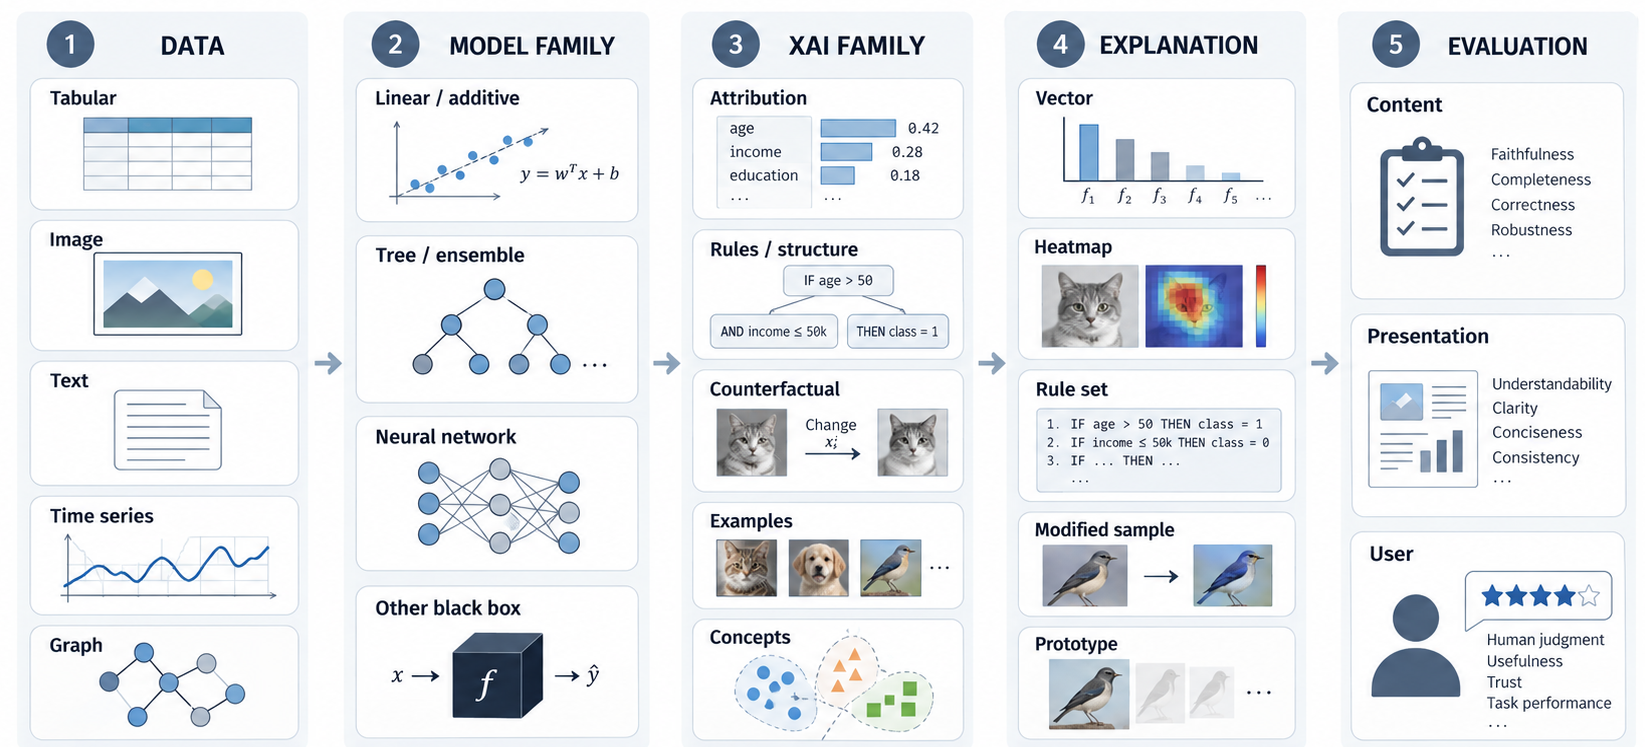
\includegraphics[width=.98\linewidth,height=.70\textheight,keepaspectratio]{xai_landscape_overview.png}
\end{frame}

\begin{frame}{Three evaluation perspectives}
\begin{description}
  \item[Functionally grounded] Computational proxies; scalable and repeatable.
  \item[Human-grounded] Simplified tasks with people; measures understanding or use.
  \item[Application-grounded] Domain experts performing a real task; costly but direct.
\end{description}
These answer different questions; one does not substitute for another.
\end{frame}

\begin{frame}{The literature uses overlapping language}
Explainability, interpretability, transparency, faithfulness, stability, robustness, comprehensibility, and actionability are related but not interchangeable.
\medskip

\centering A shared vocabulary makes claims testable.
\end{frame}

\begin{frame}{Four levels}
\centering
\includegraphics[width=.9\linewidth]{notion_property_metric.pdf}
\begin{description}
  \item[Notion] Broad conceptual idea.
  \item[Property] Desired quality of an explanation.
  \item[Metric] Formal operationalization.
  \item[Measurement] Observed value under a protocol.
\end{description}
\end{frame}

\begin{frame}{From property to measurement}
\begin{block}{Claim} The explanation is faithful to the predictive model.
\end{block}
\begin{block}{One operationalization} Deletion AUC; replace top-ranked features by the training median.
\end{block}
\begin{block}{Measurement} 0.31 on a named model, dataset, target, baseline, and seed.
\end{block}
A scalar without its protocol is incomplete evidence.
\end{frame}

\begin{frame}{The evaluation chain}
\[
\boxed{\text{Goal}\to\text{Claim}\to\text{Property}\to\text{Metric}\to\text{Protocol}\to\text{Evidence}}
\]
The metric is selected after the claim and property, not before them.
\end{frame}

\begin{frame}{Co-12: a quality map, not a scorecard}
\centering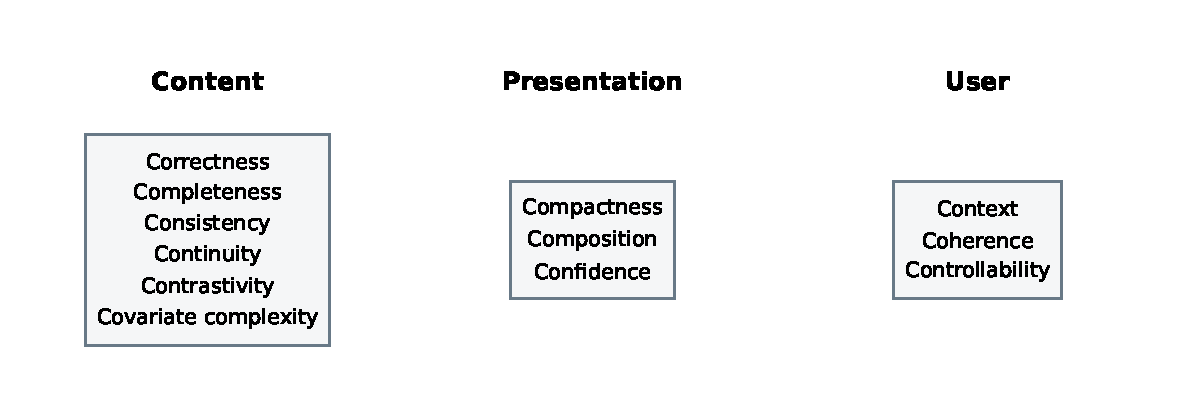
\includegraphics[width=.88\linewidth]{co12_structure.pdf}
\small Based on the Content, Presentation, and User organization in the evaluation literature.\cite{nauta}
\end{frame}

\begin{frame}{Co-12: questions to ask}
\small
\begin{tabular}{ll}
\toprule
Content & Presentation / User\\
\midrule
Correctness & Compactness: concise enough?\\
Completeness & Composition: appropriate form?\\
Consistency, continuity & Confidence: uncertainty represented?\\
Contrastivity & Context: useful for this task?\\
Covariate complexity & Coherence: aligns with domain knowledge?\\
 & Controllability: user can interact?\\
\bottomrule
\end{tabular}
\end{frame}

\begin{frame}{One property, multiple metrics}
\begin{center}
Correctness / faithfulness\\[.5em]
\begin{tabular}{ccc}
Deletion & Faithfulness correlation & Infidelity\\
Insertion & Randomization checks & Synthetic / white-box checks
\end{tabular}
\end{center}
Different operationalizations expose different assumptions and failure modes.\cite{quantus}
\end{frame}

\begin{frame}{Properties can conflict}
\centering\Large A faithful explanation may be verbose.\\[.6em]
A compact explanation may omit relevant behavior.\\[.6em]
\normalsize The evaluation objective must state which trade-offs are acceptable.
\end{frame}

\begin{frame}{Faithful does not imply understandable}
\PerspectiveTag{\ContentIcon}{Content}\hfill \PerspectiveTag{\PresentationIcon}{Presentation}

\vspace{.4em}
\[
\text{Faithful}\not\Rightarrow\text{Understandable}
\]
A technically faithful explanation with a large number of predicates may be unusable for its audience.
\end{frame}

\begin{frame}{Plausible does not imply faithful}
\PerspectiveTag{\UserIcon}{User}\hfill \PerspectiveTag{\ContentIcon}{Content}

\vspace{.4em}
\[
\text{Coherent with human knowledge}\not\Rightarrow\text{Correct relative to model}
\]
A domain expert may find an explanation plausible even if the model relies on a spurious feature.
\end{frame}

\begin{frame}{Human-grounded tasks}
\PerspectiveTag{\UserIcon}{User}\hfill Coherence, context, controllability

\vspace{.4em}
\begin{itemize}
  \item Predict the model output; detect a model failure.
  \item Identify influential variables; answer comprehension questions.
  \item Measure decision time, confidence, and calibration.
\end{itemize}
Preference alone is weak evidence: ``Which explanation do you like?'' does not test task performance.
\end{frame}

\begin{frame}{Application-grounded questions}
\PerspectiveTag{\UserIcon}{User}\hfill Context and task performance

\vspace{.4em}
\begin{description}
  \item[Physician] Does the explanation support diagnosis or error detection?
  \item[Engineer] Does it help debug model behavior?
  \item[Auditor] Does it reveal unacceptable dependencies?
  \item[Scientist] Does it generate useful hypotheses?
\end{description}
\end{frame}

\begin{frame}{A reproducible teaching benchmark}
\begin{itemize}
  \item Breast Cancer Wisconsin data; training-only standardization.
  \item Logistic regression, random forest, and MLP; class-1 probability.
  \item Local replacement attribution; model-specific attribution where available; random control.
  \item Median baseline; 25 selected test cases; explicit perturbation radius.
\end{itemize}
Designed for a short class run, not state-of-the-art comparison.
\end{frame}

\begin{frame}{Metric matrix: keep directions visible}
\PerspectiveTag{\ContentIcon}{Content}\quad Faithfulness, completeness, continuity\hfill
\PerspectiveTag{\PresentationIcon}{Presentation}\quad Compactness

\vspace{.4em}
\begin{center}\small
Deletion AUC $\downarrow$\quad Faithfulness correlation $\uparrow$\\
Comprehensiveness $\uparrow$\quad Sufficiency $\downarrow$\\
Max-sensitivity $\downarrow$\quad Gini sparsity: descriptive only
\end{center}
The table and plots below are computed from per-instance benchmark outputs. Column scaling is for visual comparison, not a common utility score.
\centering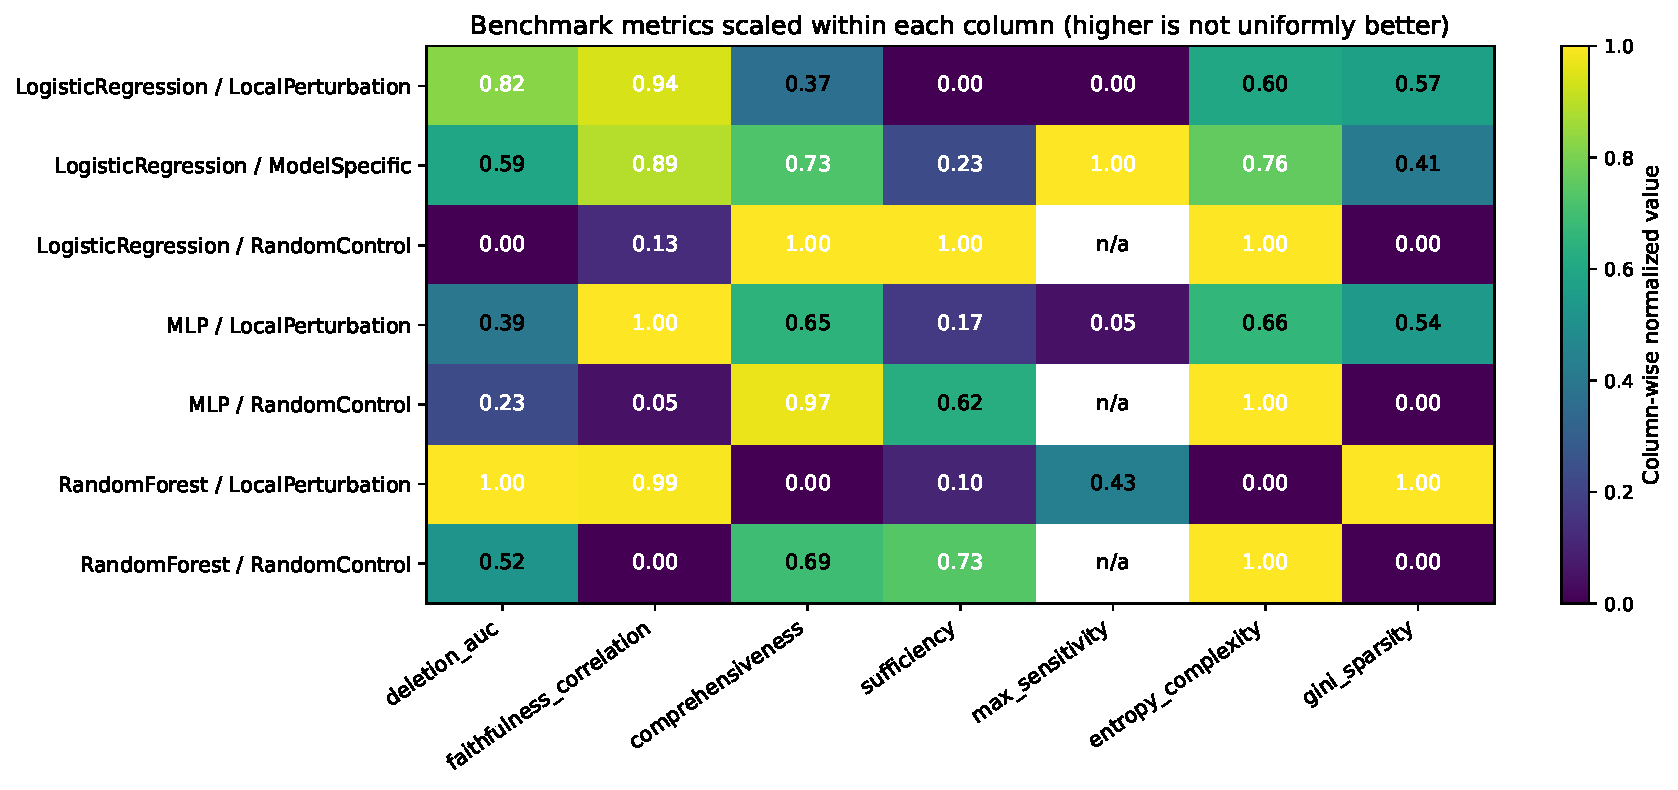
\includegraphics[width=.86\linewidth,height=.43\textheight,keepaspectratio]{benchmark_heatmap.pdf}
\end{frame}

\begin{frame}{Include negative controls}
\PerspectiveTag{\ContentIcon}{Content}\hfill Correctness / faithfulness

\vspace{.4em}
Random feature rankings and model randomization ask whether the protocol can reject explanations that should not earn high faithfulness.
\medskip

An evaluation without controls can produce precise-looking but uncalibrated scores.
\end{frame}

\begin{frame}{Metric disagreement}
\centering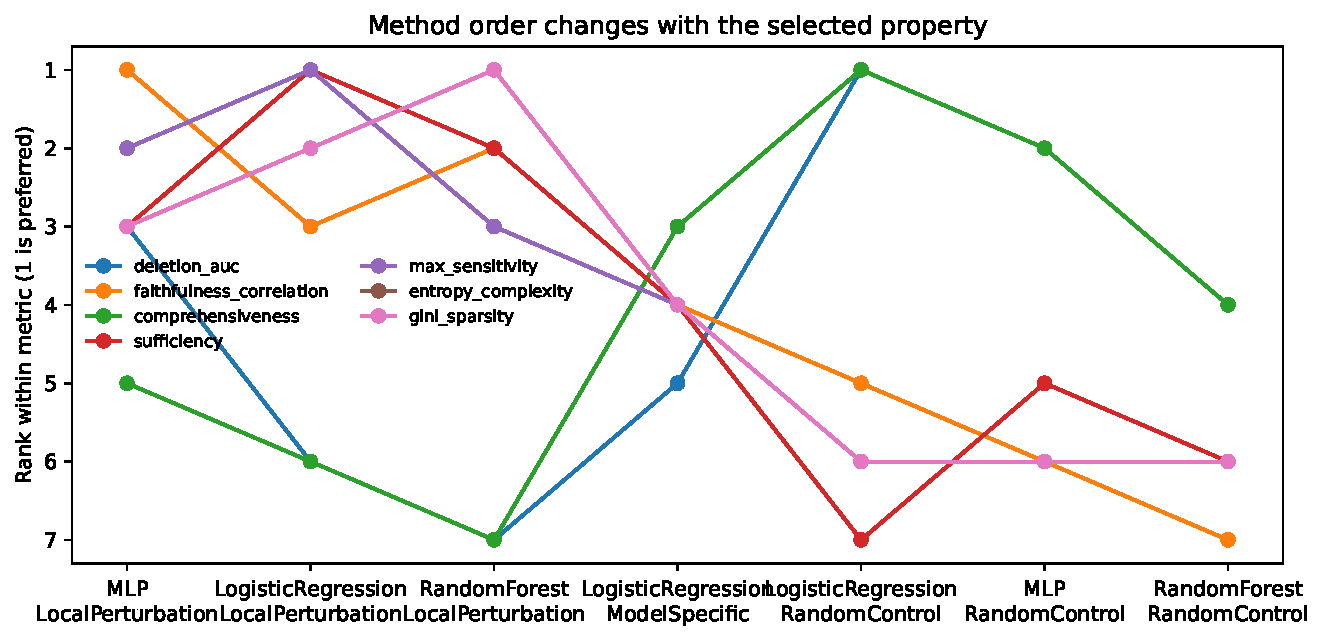
\includegraphics[width=.85\linewidth,height=.7\textheight,keepaspectratio]{rank_disagreement.pdf}
\end{frame}

\begin{frame}{Metrics do not necessarily agree}
\centering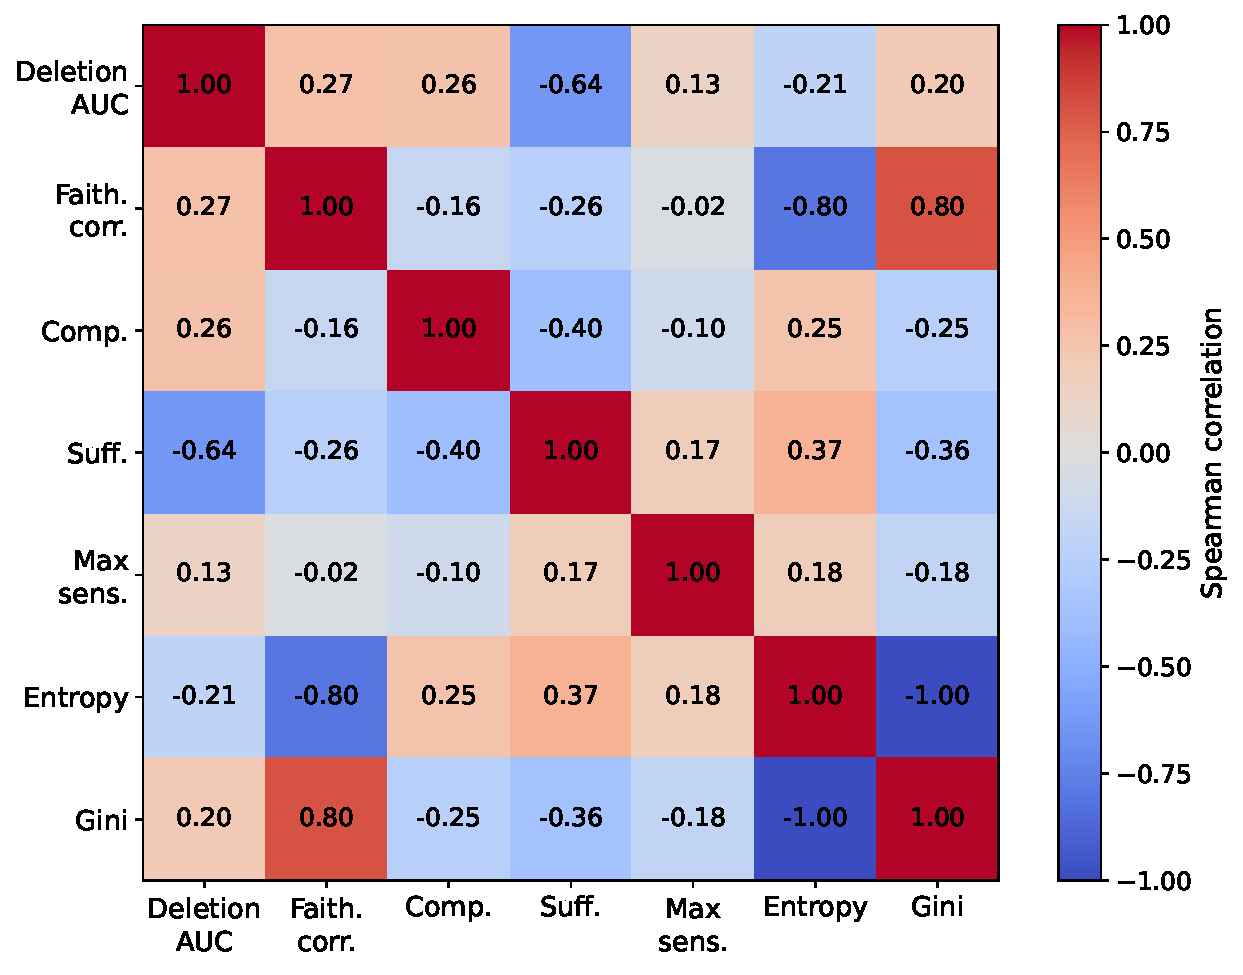
\includegraphics[width=.78\linewidth,height=.74\textheight,keepaspectratio]{metric_correlation.pdf}
Ranks and correlations describe this benchmark's models, samples, and protocol. They do not define a universal ordering.
\end{frame}

\begin{frame}{Multi-objective view}
\centering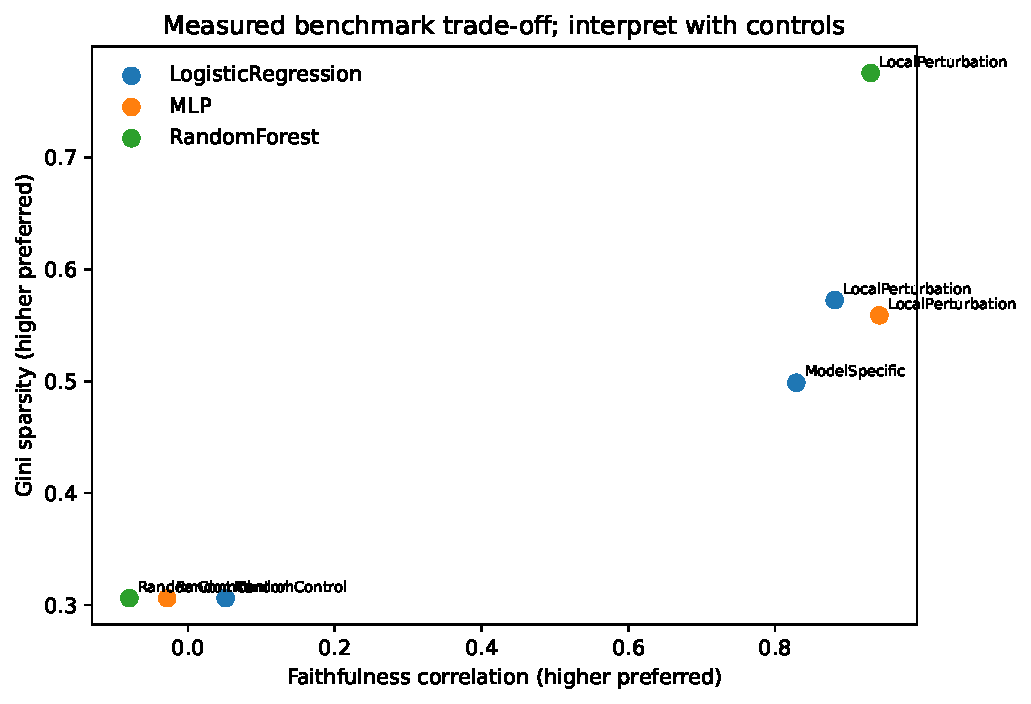
\includegraphics[width=.72\linewidth,height=.7\textheight,keepaspectratio]{pareto_xai.pdf}

\PerspectiveTag{\ContentIcon}{Content}\quad faithfulness, stability\hspace{1.4em}
\PerspectiveTag{\PresentationIcon}{Presentation}\quad compactness

Avoid aggregation until the application defines a utility.
\end{frame}

\begin{frame}{Discussion}
\PerspectiveLegend

\vspace{.4em}
\begin{itemize}
  \item Better deletion AUC but worse stability: which method is better?
  \item If deletion is out of distribution, what did the score test?
  \item What control should a benchmark be able to reject?
\end{itemize}
Answer by naming the claim and intended use.
\end{frame}

\begin{frame}{A defensible evaluation workflow}
\centering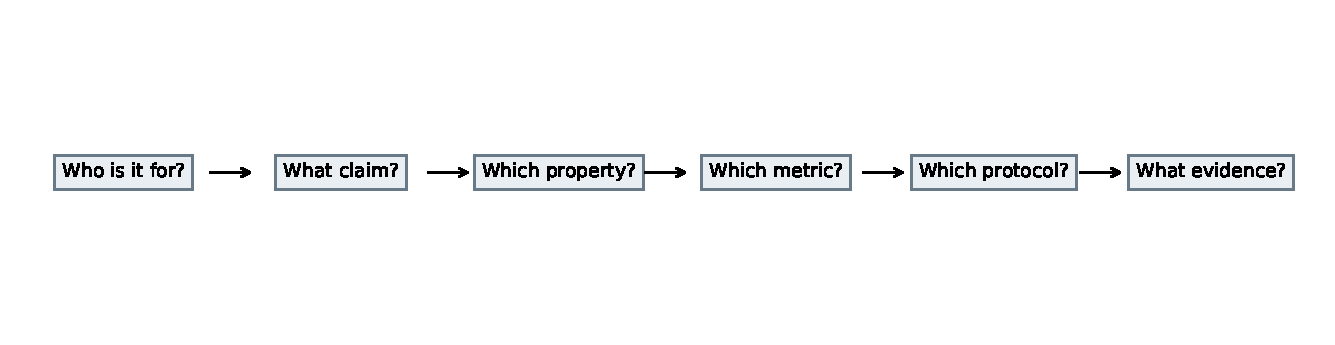
\includegraphics[width=.92\linewidth,height=.5\textheight,keepaspectratio]{evaluation_workflow.pdf}

\vspace{.8em}
{\small Then specify baselines, controls, aggregation, uncertainty, and the need for human evaluation.\par}
\end{frame}

\begin{frame}{Take-home points}
\begin{enumerate}
  \item Explanation quality is multidimensional.
  \item A property and a metric are not the same thing.
  \item Metrics encode assumptions about perturbations, baselines, and outputs.
  \item Technical validity and human usefulness are different questions.
  \item Strong evaluation combines complementary evidence and controls.
\end{enumerate}
\end{frame}

\begin{frame}{Final question}
\centering\Large Do not evaluate an explanation.\\[.5em]
Evaluate claims about an explanation.\\[1em]
\normalsize Which claim? Which property? Which metric? Which protocol? Compared with what control?
\end{frame}

\begin{frame}[allowframebreaks]{References}
\bibliographystyle{abbrv}
\bibliography{references}
\end{frame}
\appendix
\begin{frame}{Faithfulness: perturb important features}
\HierarchyHeader{\ContentIcon}{Content}{Correctness / faithfulness}{Do important attributed features control the model output?}
Let $a=E(f,x)$, where $a_i$ is feature importance. A perturbation-based test asks whether replacing features with large $|a_i|$ changes $f(x)$.
\[
\Delta_i=f(x)-f(\xdel{i})
\]
Here $\xdel{i}$ denotes $x$ with feature $i$ replaced by the chosen baseline. The replacement rule is part of the metric.
\end{frame}

\begin{frame}{Faithfulness correlation}
\HierarchyHeader{\ContentIcon}{Content}{Correctness / faithfulness}{Does attribution mass correlate with output change?}
\[
\operatorname{FC}(x)=\operatorname{corr}_{S}\left(\sum_{i\in S}a_i,\; f(x)-f(\xdel{S})\right)
\]
Positive association is evidence that attribution mass tracks output change under the sampled subsets and replacement protocol.
\end{frame}

\begin{frame}{Deletion curve}
\HierarchyHeader{\ContentIcon}{Content}{Correctness / faithfulness}{What happens when top-ranked features are removed first?}
Rank features by $|a_i|$, then progressively replace the most important ones. A steep score decrease early in the curve is consistent with a useful ranking under this deletion rule.
\centering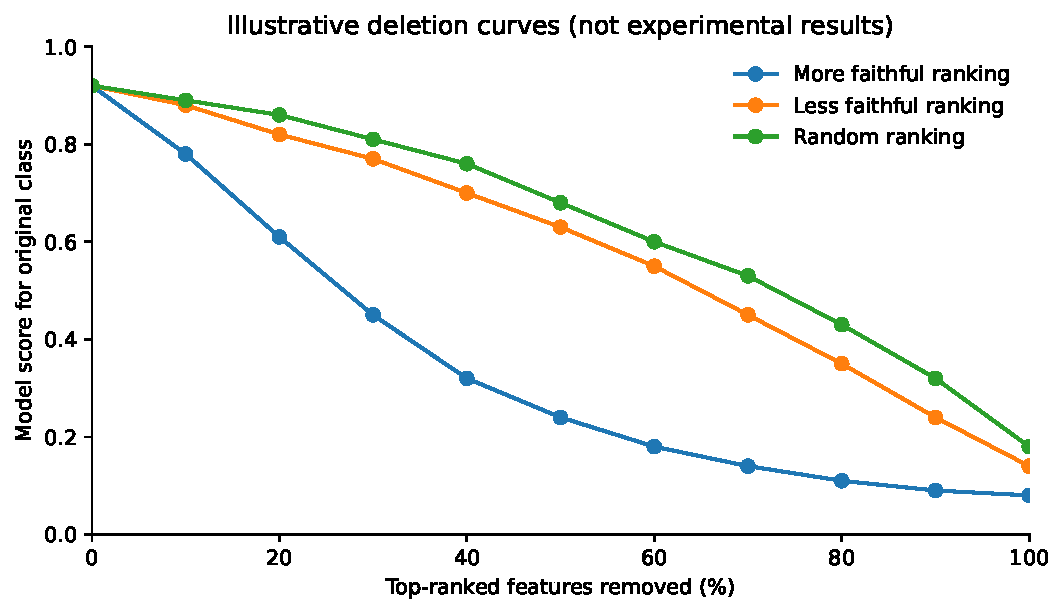
\includegraphics[width=.7\linewidth,height=.46\textheight,keepaspectratio]{deletion_curve.pdf}
\end{frame}

\begin{frame}{Deletion AUC and AOPC}
\HierarchyHeader{\ContentIcon}{Content}{Correctness / faithfulness}{How do we summarize a deletion trajectory?}
\[
\mathrm{AUC}_{del}=\int_0^1 f(\xdel{\alpha})\,d\alpha
\qquad
\mathrm{AOPC}_{del}=\frac1K\sum_{k=1}^K\left[f(x)-f(\xdel{k})\right]
\]
\centering
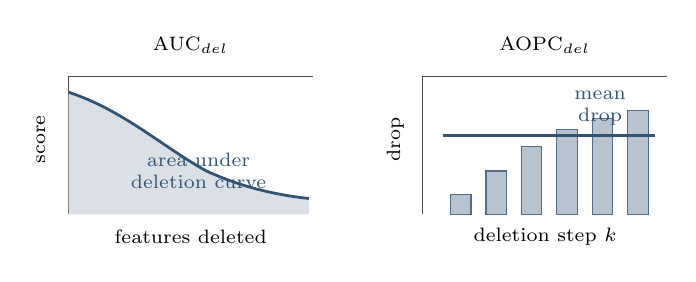
\begin{tikzpicture}[x=1cm,y=1cm,>=stealth]
\tikzset{axis/.style={draw=black!70,line width=.35pt}, lab/.style={font=\scriptsize,align=center}}
\begin{scope}[shift={(0,0)}]
  \node[lab,font=\bfseries\scriptsize] at (1.55,2.15) {$\mathrm{AUC}_{del}$};
  \draw[axis] (0,0) -- (0,1.75) -- (3.1,1.75);
  \node[lab,rotate=90] at (-.35,.95) {score};
  \node[lab] at (1.55,-.28) {features deleted};
  \fill[contentblue!18] (0,0) -- (0,1.55) .. controls (.7,1.32) and (1.2,.85) .. (1.75,.55)
    .. controls (2.25,.32) and (2.7,.24) .. (3.05,.2) -- (3.05,0) -- cycle;
  \draw[contentblue,line width=1pt] (0,1.55) .. controls (.7,1.32) and (1.2,.85) .. (1.75,.55)
    .. controls (2.25,.32) and (2.7,.24) .. (3.05,.2);
  \node[lab,contentblue] at (1.65,.55) {area under\\deletion curve};
\end{scope}
\begin{scope}[shift={(4.5,0)}]
  \node[lab,font=\bfseries\scriptsize] at (1.55,2.15) {$\mathrm{AOPC}_{del}$};
  \draw[axis] (0,0) -- (0,1.75) -- (3.1,1.75);
  \node[lab,rotate=90] at (-.35,.95) {drop};
  \node[lab] at (1.55,-.28) {deletion step $k$};
  \foreach \x/\h in {.35/.25,.8/.55,1.25/.86,1.7/1.08,2.15/1.22,2.6/1.32}
    \draw[fill=contentblue!35,draw=contentblue!85] (\x,0) rectangle +(0.26,\h);
  \draw[contentblue,line width=1pt] (.25,1.0) -- (2.95,1.0);
  \node[lab,contentblue] at (2.25,1.35) {mean\\drop};
\end{scope}
\end{tikzpicture}

\vspace{.4em}
\raggedright\small For a score-preserving output and a fixed deletion rule, lower deletion AUC or higher AOPC is generally preferred. Always state direction and target output.
\end{frame}

\begin{frame}{Comprehensiveness and sufficiency}
\HierarchyHeader{\ContentIcon}{Content}{Completeness}{Is the selected evidence enough, and is removing it consequential?}
\[
\mathrm{Comp}(x,S)=f(x)-f(\xdel{S})\qquad
\mathrm{Suff}(x,S)=|f(x)-f(\xkeep{S})|
\]
\begin{itemize}
  \item Remove selected features: does the score change? Higher drop is generally preferred.
  \item Keep selected features: does the score remain? Smaller difference is generally preferred.
\end{itemize}
\centering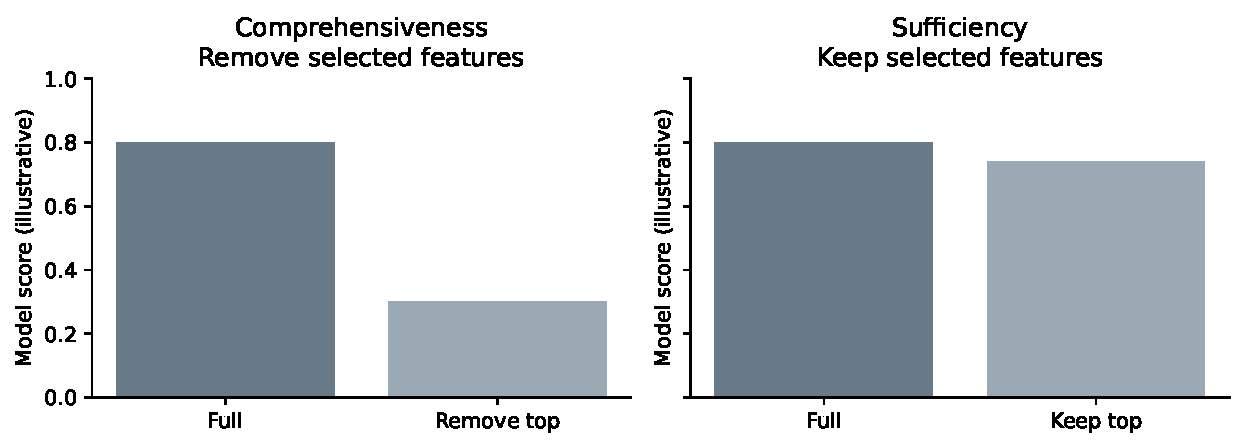
\includegraphics[width=.66\linewidth,height=.3\textheight,keepaspectratio]{comprehensiveness_sufficiency.pdf}
\end{frame}

\begin{frame}{Infidelity}
\HierarchyHeader{\ContentIcon}{Content}{Correctness / faithfulness}{Does the attribution-predicted change match the real change?}
\[
\operatorname{Infid}(E,f,x)=\mathbb{E}_{\delta}\left[\left(\delta^\top E(f,x)-\left(f(x)-f(x-\delta)\right)\right)^2\right]
\]
\centering
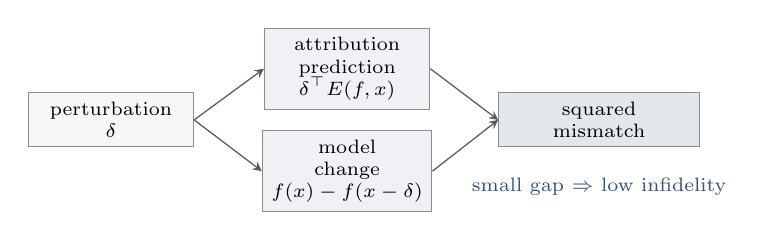
\begin{tikzpicture}[x=1cm,y=1cm,>=stealth]
\tikzset{
  box/.style={draw=black!45,fill=black!3,minimum width=2.1cm,minimum height=.58cm,align=center,font=\scriptsize},
  lab/.style={font=\scriptsize,align=center},
  arr/.style={->,draw=black!65,line width=.45pt}
}
\node[box] (pert) at (0,1.1) {perturbation\\$\delta$};
\node[box,fill=contentblue!8] (pred) at (3.0,1.75) {attribution\\prediction\\$\delta^\top E(f,x)$};
\node[box,fill=contentblue!8] (actual) at (3.0,.45) {model\\change\\$f(x)-f(x-\delta)$};
\node[box,fill=contentblue!14,minimum width=2.55cm] (gap) at (6.2,1.1) {squared\\mismatch};
\draw[arr] (pert.east) -- (pred.west);
\draw[arr] (pert.east) -- (actual.west);
\draw[arr] (pred.east) -- (gap.west);
\draw[arr] (actual.east) -- (gap.west);
\node[lab,contentblue] at (6.2,.25) {small gap $\Rightarrow$ low infidelity};
\end{tikzpicture}

\vspace{.35em}
\raggedright\small
It compares attribution-predicted change with actual model change. The perturbation distribution over $\delta$ defines what changes are tested.\cite{infidelity}
\end{frame}

\begin{frame}{The perturbation problem}
\HierarchyHeader{\ContentIcon}{Content}{Measurement validity}{Does the perturbation still represent a meaningful input?}
\centering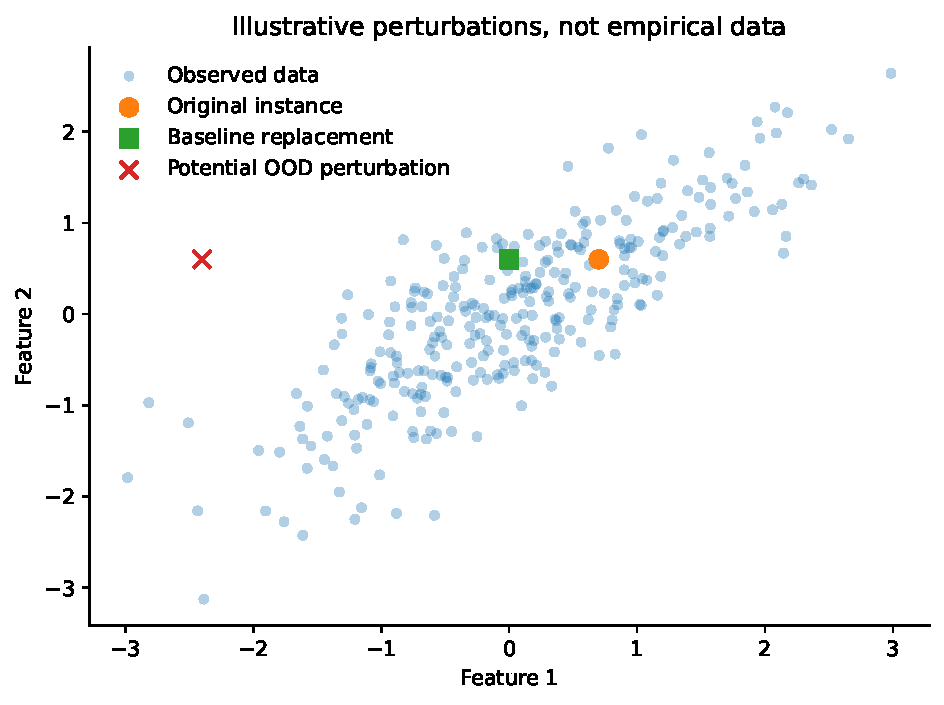
\includegraphics[width=.5\linewidth,height=.45\textheight,keepaspectratio]{ood_perturbation.pdf}
\begin{itemize}
  \item What does ``feature absence'' mean: zero, mean, median, or conditional sample?
  \item If replacement leaves the data manifold, are we measuring the explanation or model extrapolation?
\end{itemize}
\end{frame}

\begin{frame}{Baseline sensitivity is a result}
\HierarchyHeader{\ContentIcon}{Content}{Measurement validity}{How much does the score depend on the replacement convention?}
\centering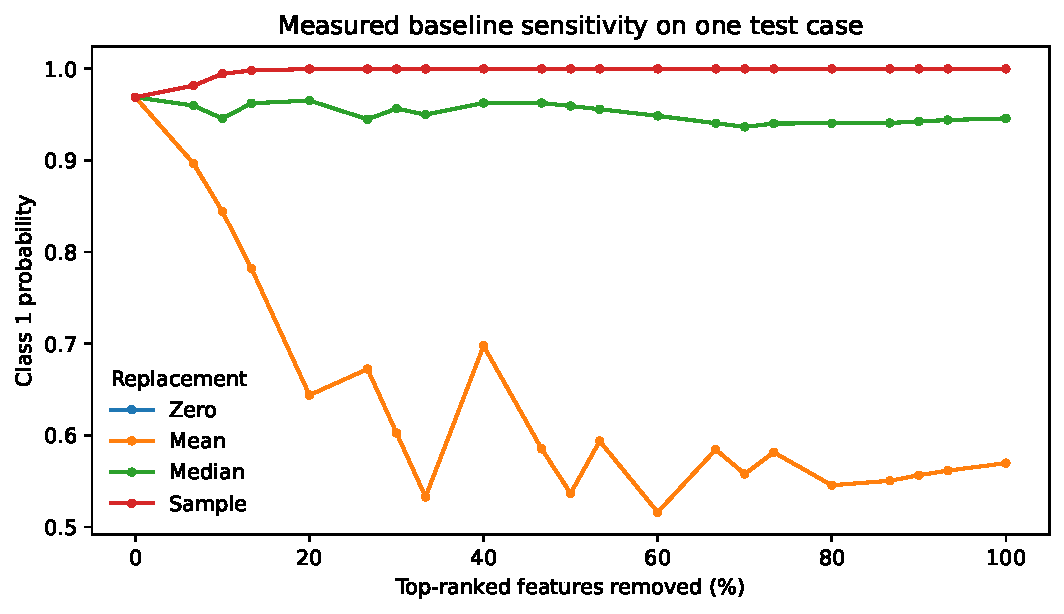
\includegraphics[width=.74\linewidth,height=.55\textheight,keepaspectratio]{baseline_sensitivity.pdf}
\small Measured on one held-out instance; the curve changes when the replacement convention changes.
\end{frame}

\begin{frame}{Consistency is not continuity}
\HierarchyHeader{\ContentIcon}{Content}{Consistency / continuity}{Are we testing repeatability or local stability?}
\begin{description}
  \item[Consistency] Equivalent input/model conditions yield equivalent explanations.
  \item[Continuity] Similar inputs with similar predictions yield similar explanations.
\end{description}
Repeated seeds and equivalent implementations probe consistency; nearby inputs probe continuity.
\end{frame}

\begin{frame}{Max-sensitivity}
\HierarchyHeader{\ContentIcon}{Content}{Continuity}{How much can the explanation change in a small neighborhood?}
\[
\mathrm{Sens}_{max}=\max_{\|x'-x\|\le r}\|E(f,x)-E(f,x')\|
\]
The radius, input norm, explanation distance, and validity of perturbed inputs all matter.
\centering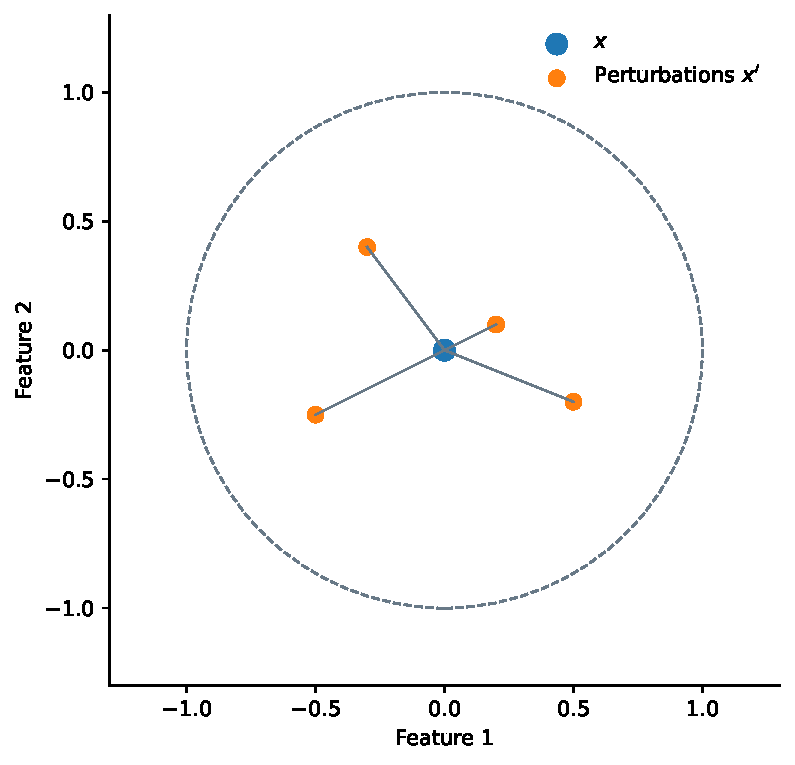
\includegraphics[width=.3\linewidth,height=.34\textheight,keepaspectratio]{robustness_neighborhood.pdf}
\end{frame}

\begin{frame}{Compactness is not correctness}
\TradeoffHeader{\PresentationIcon}{Presentation}{Compactness}{\ContentIcon}{Content}{Correctness / faithfulness}{A concise explanation is easier to inspect, not automatically more faithful.}
\[
a=[0.91,0.04,0.03,0.01,0.01]\qquad b=[0.21,0.20,0.20,0.20,0.19]
\]
\centering Which is easier to inspect? Does that make it more faithful?\\
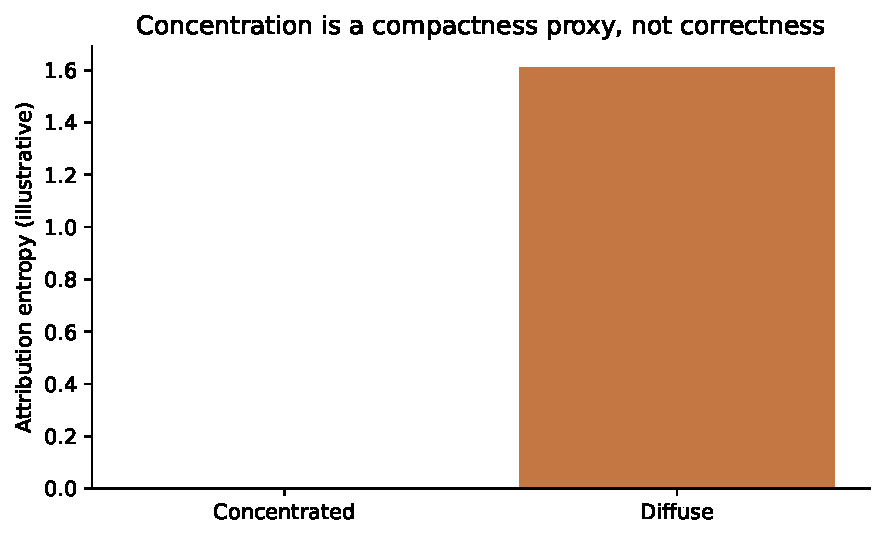
\includegraphics[width=.52\linewidth,height=.34\textheight,keepaspectratio]{complexity_examples.pdf}
\end{frame}

\begin{frame}{Entropy and sparsity}
\HierarchyHeader{\PresentationIcon}{Presentation}{Compactness}{How concentrated is the attribution representation?}
Normalize $p_i=|a_i|/\sum_j|a_j|$ and compute
\[
H(a)=-\sum_i p_i\log p_i.
\]
Lower entropy indicates concentration; higher Gini indicates concentration. Neither establishes that the explanation is correct or useful.
\end{frame}

\begin{frame}{Sanity checks}
\HierarchyHeader{\ContentIcon}{Content}{Correctness / faithfulness}{Can the protocol reject explanations that should fail?}
\centering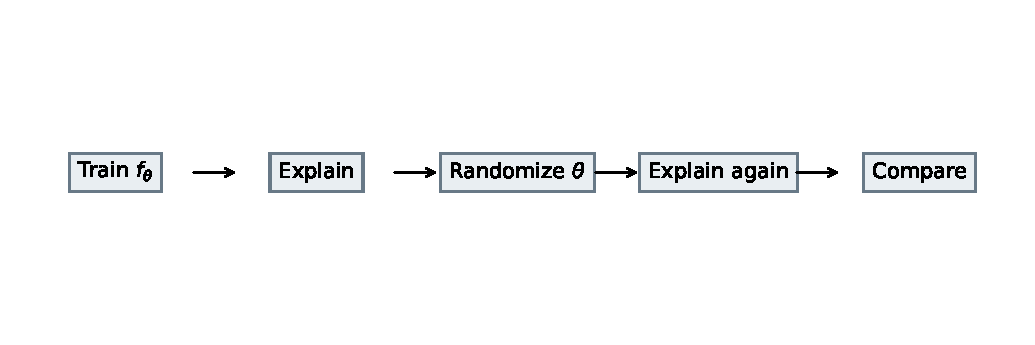
\includegraphics[width=.86\linewidth,height=.42\textheight,keepaspectratio]{randomization_check.pdf}
If explanations barely change after model parameter randomization, model dependence is questionable. Passing a sanity check is necessary evidence, not proof of correctness.\cite{sanity}
\end{frame}

\begin{frame}{Faithful does not imply understandable}
\TradeoffHeader{\ContentIcon}{Content}{Correctness / faithfulness}{\PresentationIcon}{Presentation}{Compactness / composition}{Model-relative validity and human readability are different claims.}
\[
\text{Faithful}\not\Rightarrow\text{Understandable}
\]
A technically faithful explanation with a large number of predicates may be unusable for its audience.
\end{frame}

\begin{frame}{Plausible does not imply faithful}
\TradeoffHeader{\UserIcon}{User}{Coherence}{\ContentIcon}{Content}{Correctness / faithfulness}{Human plausibility is not evidence that the explanation tracks the model.}
\[
\text{Coherent with human knowledge}\not\Rightarrow\text{Correct relative to model}
\]
A domain expert may find an explanation plausible even if the model relies on a spurious feature.
\end{frame}

\begin{frame}{Human-grounded tasks}
\HierarchyHeader{\UserIcon}{User}{Coherence / context / controllability}{Does the explanation improve a controlled human task?}
\begin{itemize}
  \item Predict the model output; detect a model failure.
  \item Identify influential variables; answer comprehension questions.
  \item Measure decision time, confidence, and calibration.
\end{itemize}
Preference alone is weak evidence: ``Which explanation do you like?'' does not test task performance.
\end{frame}

\end{document}
